%%
%% Author: Dario Chinelli
%% begin 2019-12-04
%% last mod 2022-02-02
%%

% Preamble
\documentclass[class=article, crop=false]{standalone}

% Packages
\usepackage[subpreambles=true]{standalone}
\usepackage{import}
\usepackage{graphicx}
\usepackage{amsmath}

% Document
\begin{document}
The aim of this paragraph is the comparison between the real dataset utilized to produce the models and some simulations.
The following quantities are taken into account to compare the results.
Those are plotted as histograms, to empathize the statistical approach.
\begin{enumerate}[label=(\roman*)]
\item The magnitude of the velocity vector along the $\vec x$ axes, plotted as 1-dimensional histogram;
\item the magnitude of the velocity vector along the $\vec y$ axes, plotted as 1-dimensional histogram;
\item the correlation between the position along the $\vec x$ axes and the magnitude of the velocity vector along the same axes, plotted as heat-map or 2-dimensional histogram;
\item the correlation between the position along the $\vec y$ axes and the magnitude of the velocity vector along the same axes, plotted as heat-map or 2-dimensional histogram.
\item the heat-map of the positions along $\vec x$ and $\vec y$ axis of all paths that have passed though, plotted as 2-dimensional histogram;
\end{enumerate}

\FloatBarrier
\subsection{Real data - D2Q9}







\begin{figure}[ht]
\begin{minipage}[c]{0.2\linewidth}
\centering
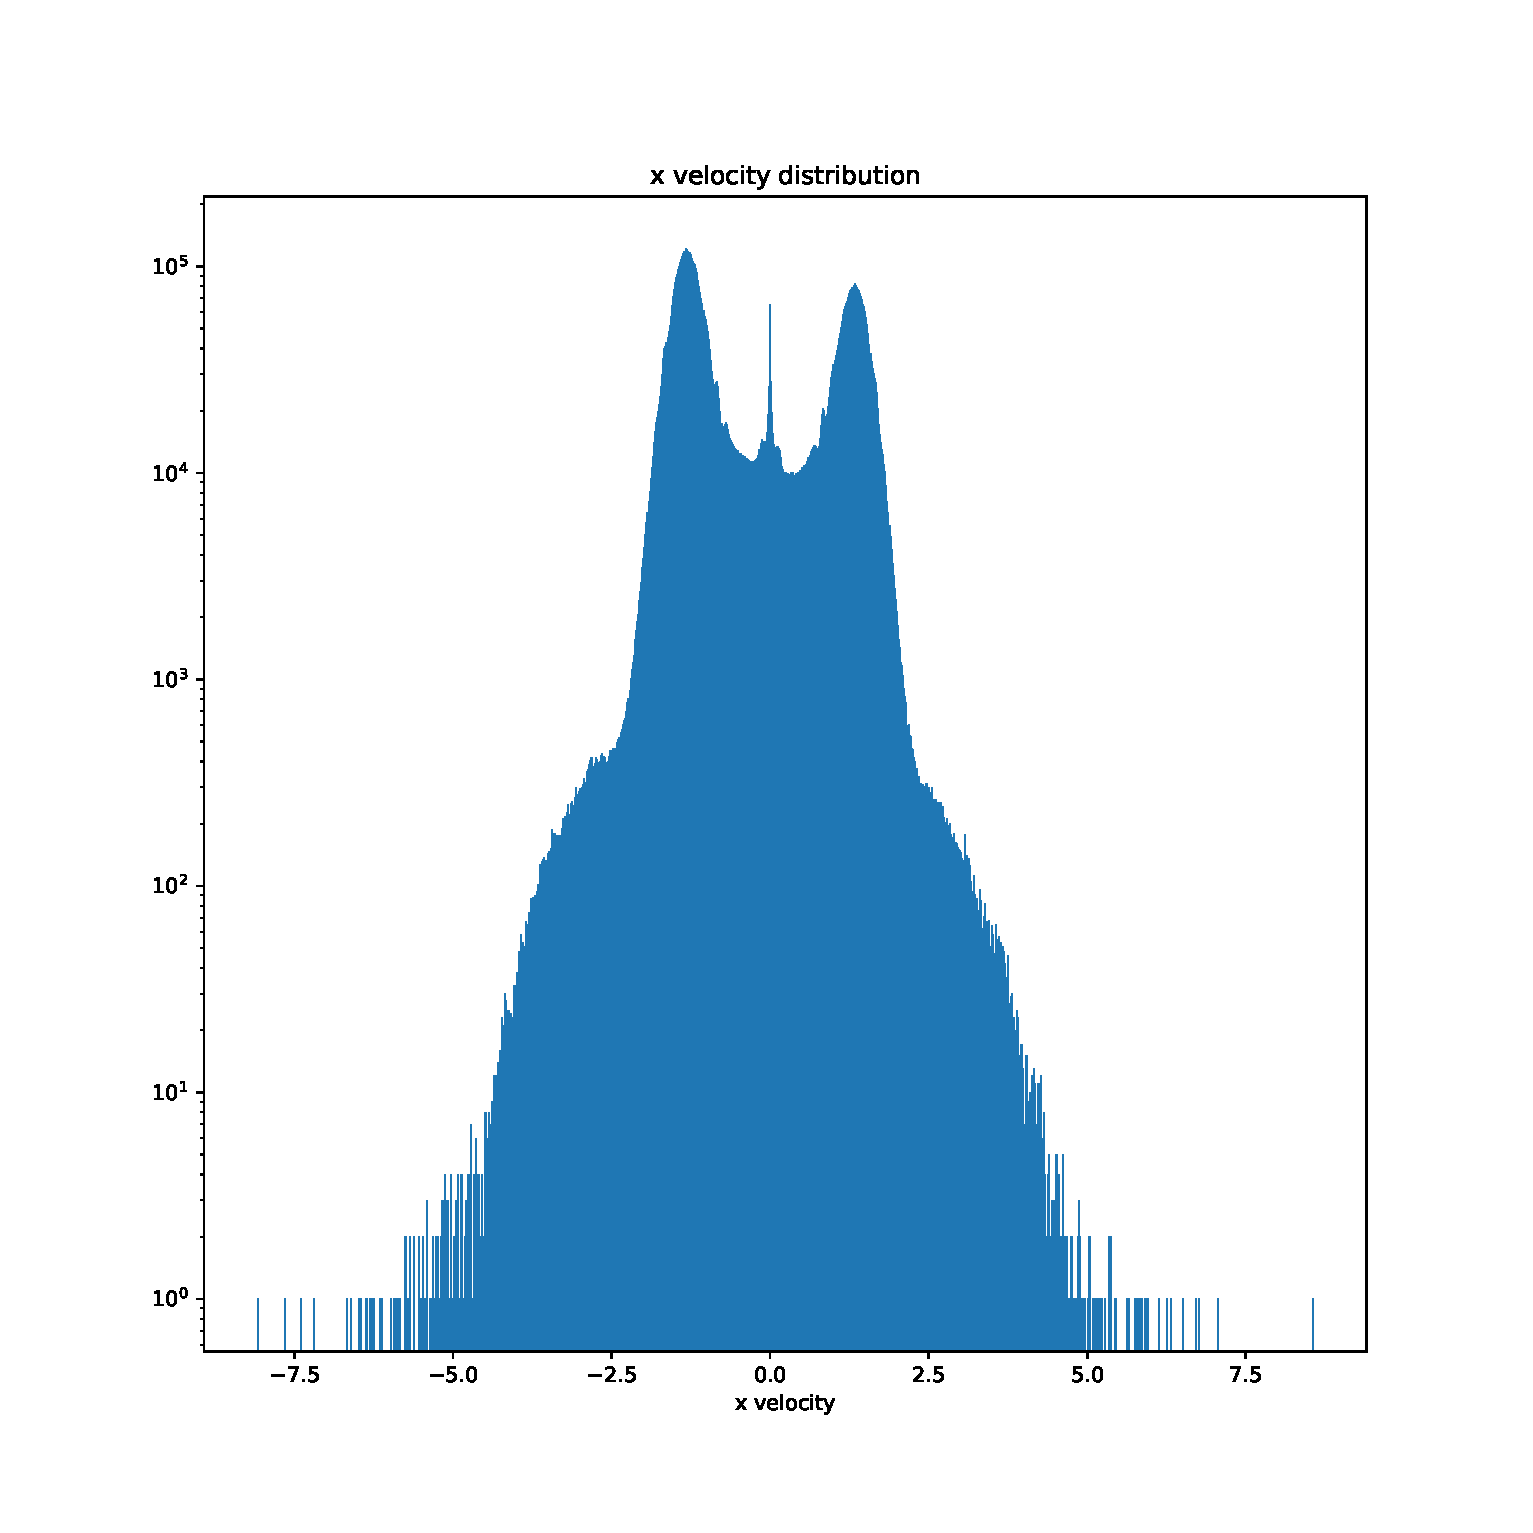
\includegraphics[ width=0.5\textwidth]{fig/hist_vx/save_trainf10_pro_RealData_hist_vx}
\captionsetup{width=.8\linewidth}
\caption{CAPTION ONE}
\label{fig:Vx_Real_i}
\end{minipage}

\begin{minipage}[c]{0.2\linewidth}
\centering
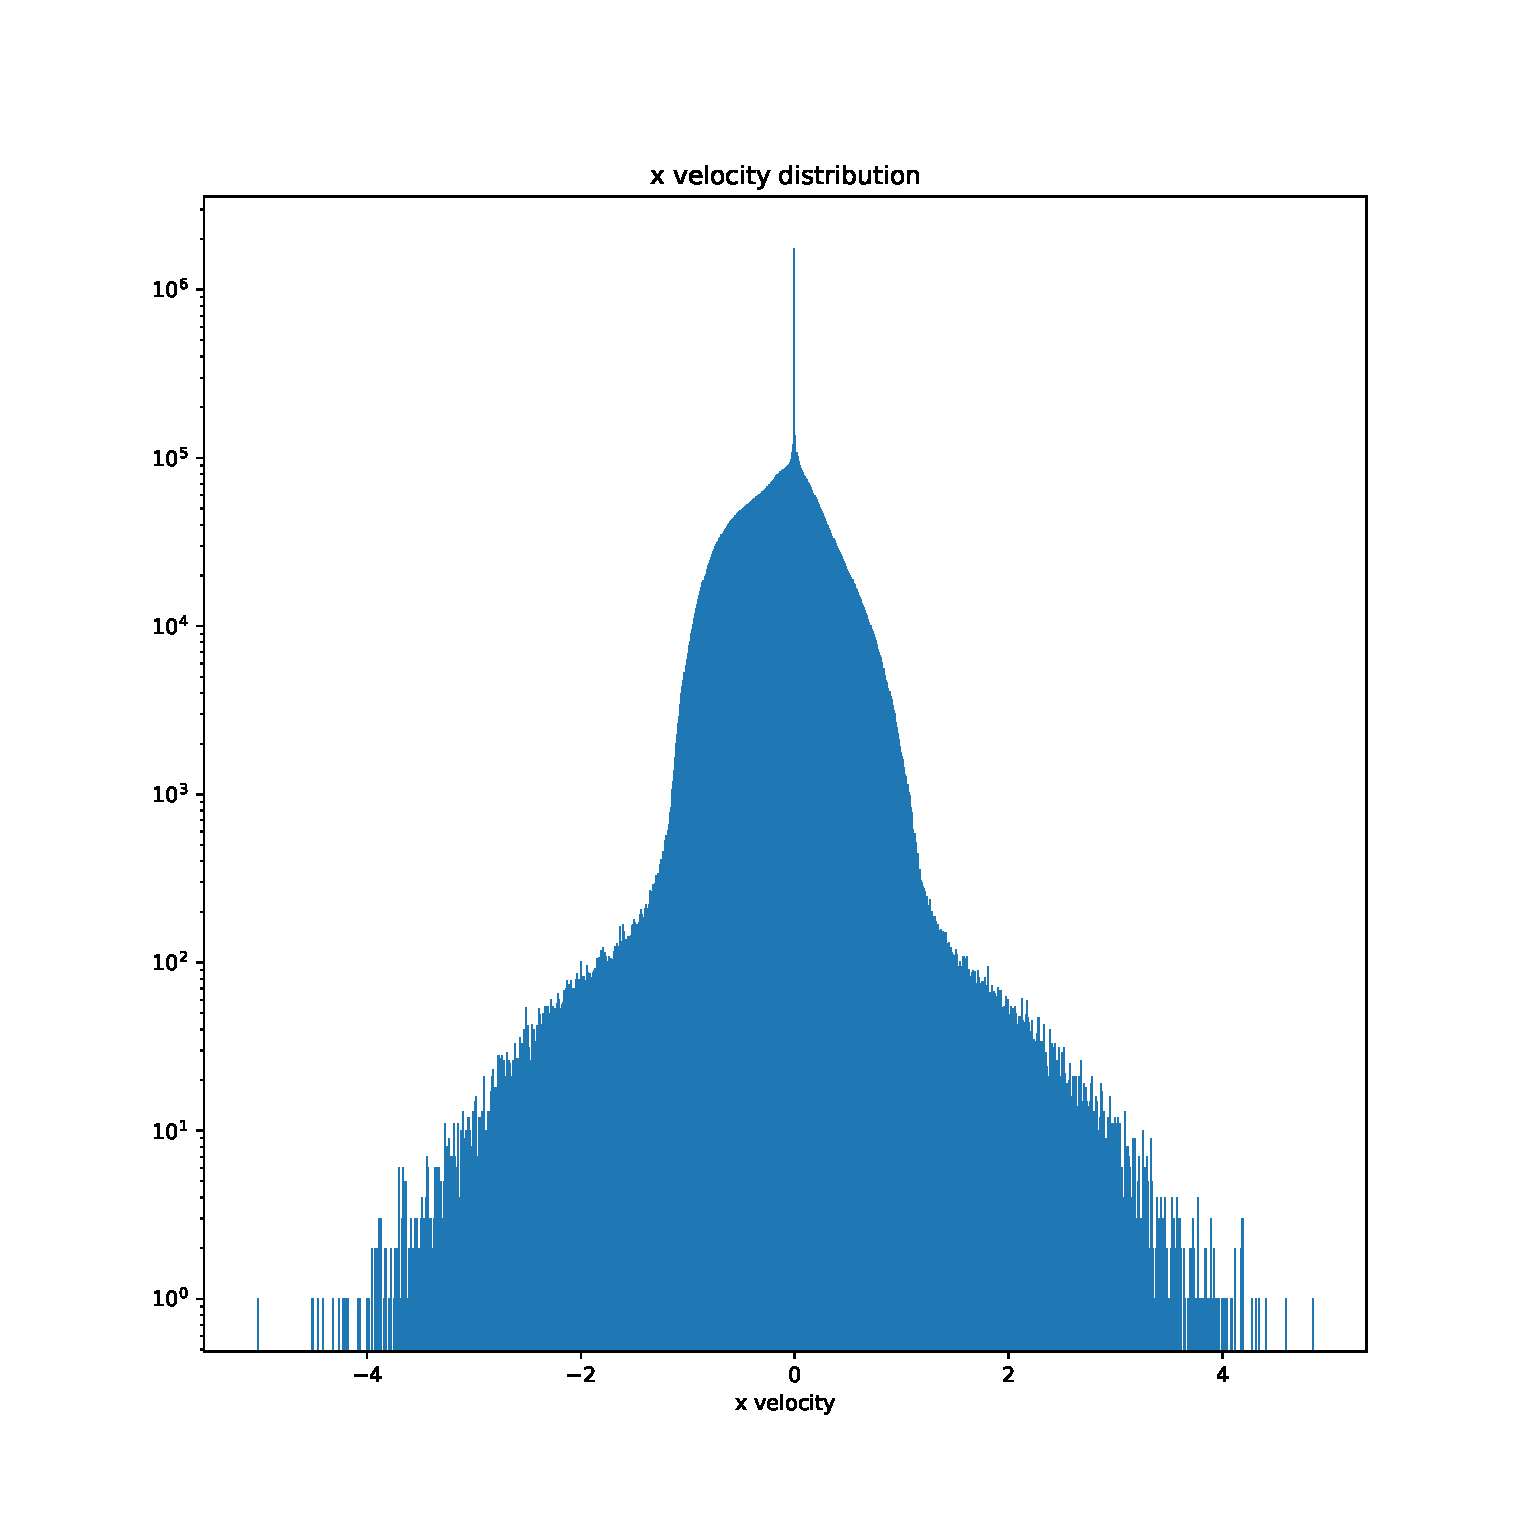
\includegraphics[ width=0.5\textwidth]{/fig/hist_vx/save_trainf10_pro_simD2Q9_hist_vx}
\captionsetup{width=.8\linewidth}
\caption{CAPTION ONE}
\label{fig:Vx_SimD2Q9}
\end{minipage}

\begin{minipage}[c]{0.2\linewidth}
\centering
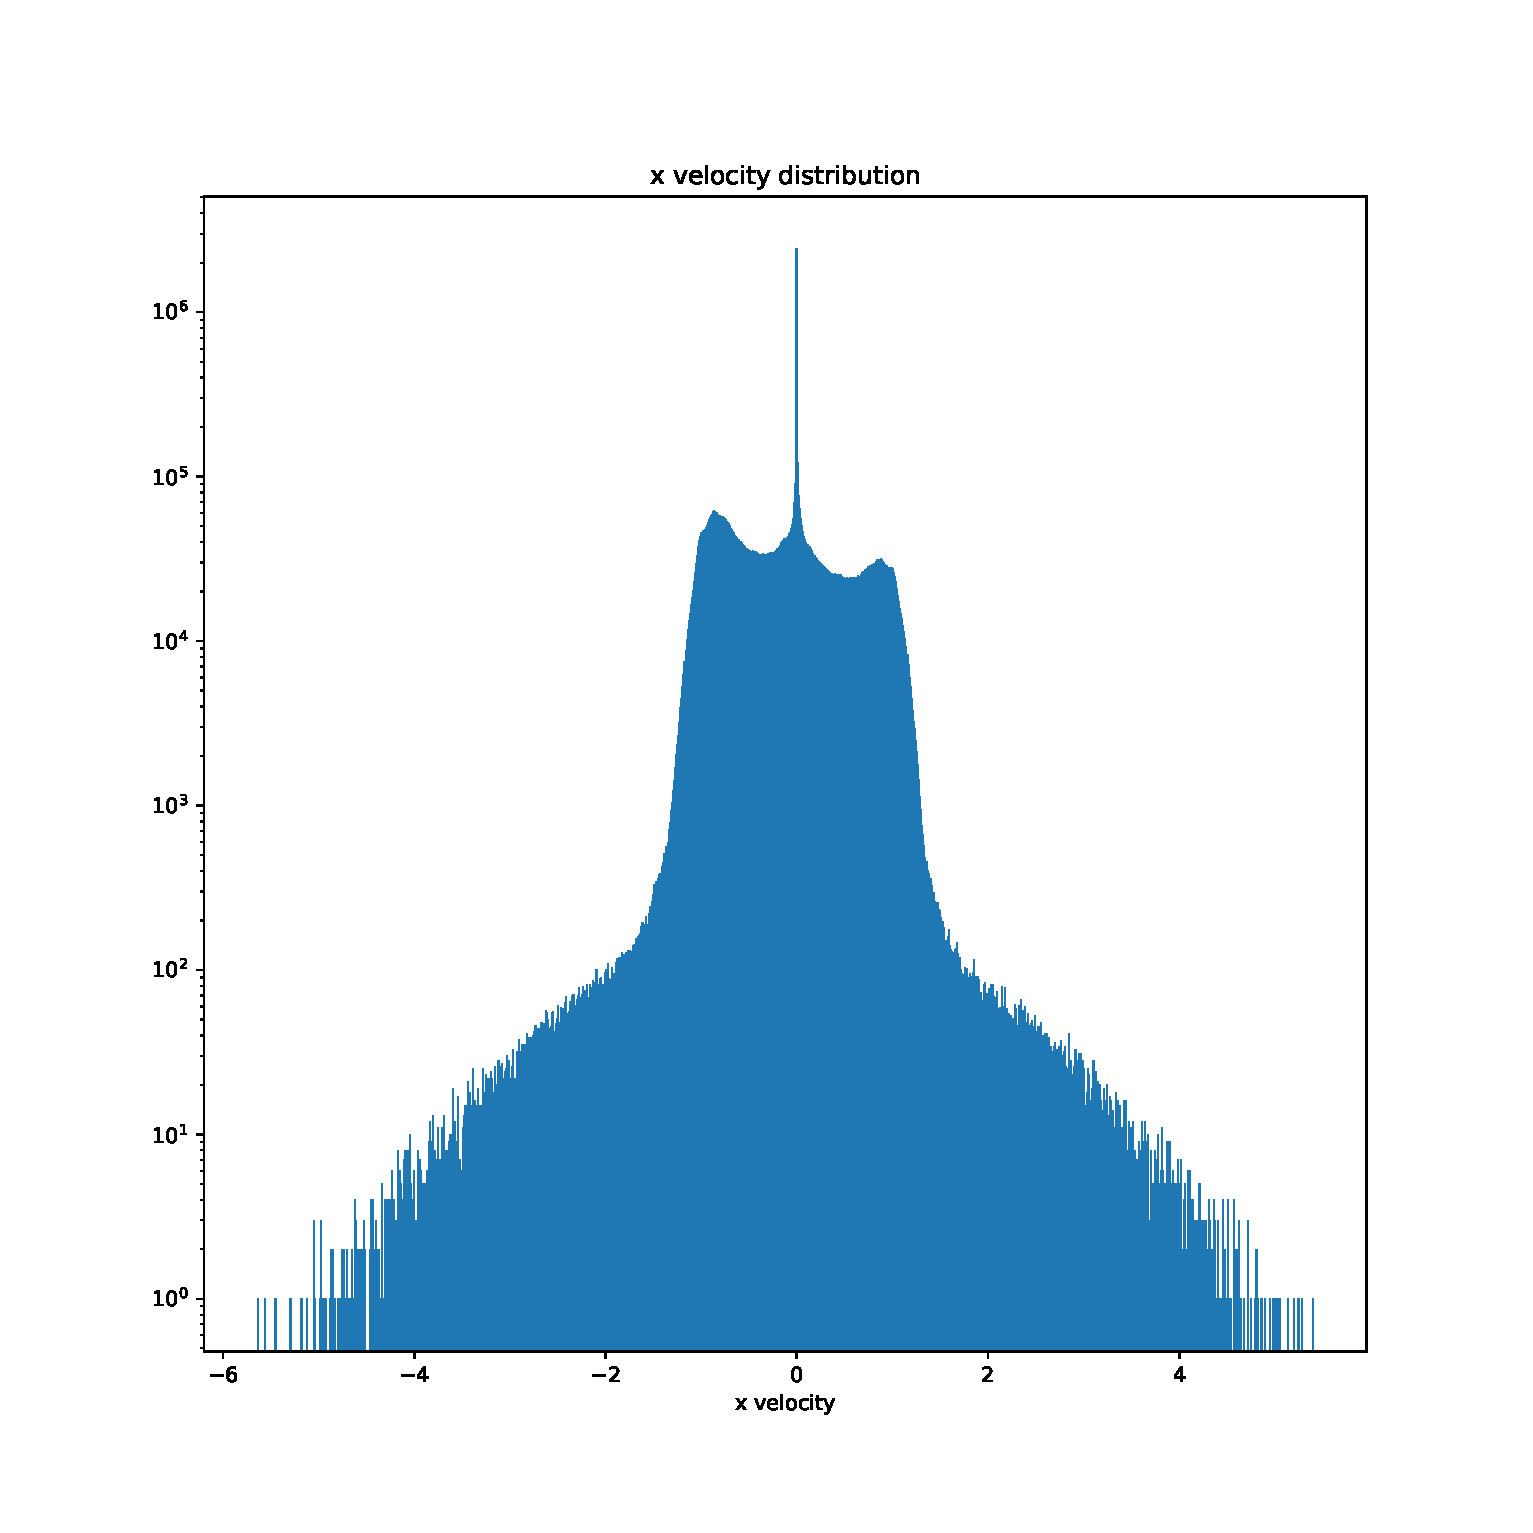
\includegraphics[ width=0.5\textwidth]{//fig/hist_vx/save_trainf10_pro_simD2Q9Q9_hist_vx}
\captionsetup{width=.8\linewidth}
\caption{CAPTION ONE}
\label{fig:Vx_SimD2Q9Q9}
\end{minipage}

\begin{minipage}[c]{0.2\linewidth}
\centering
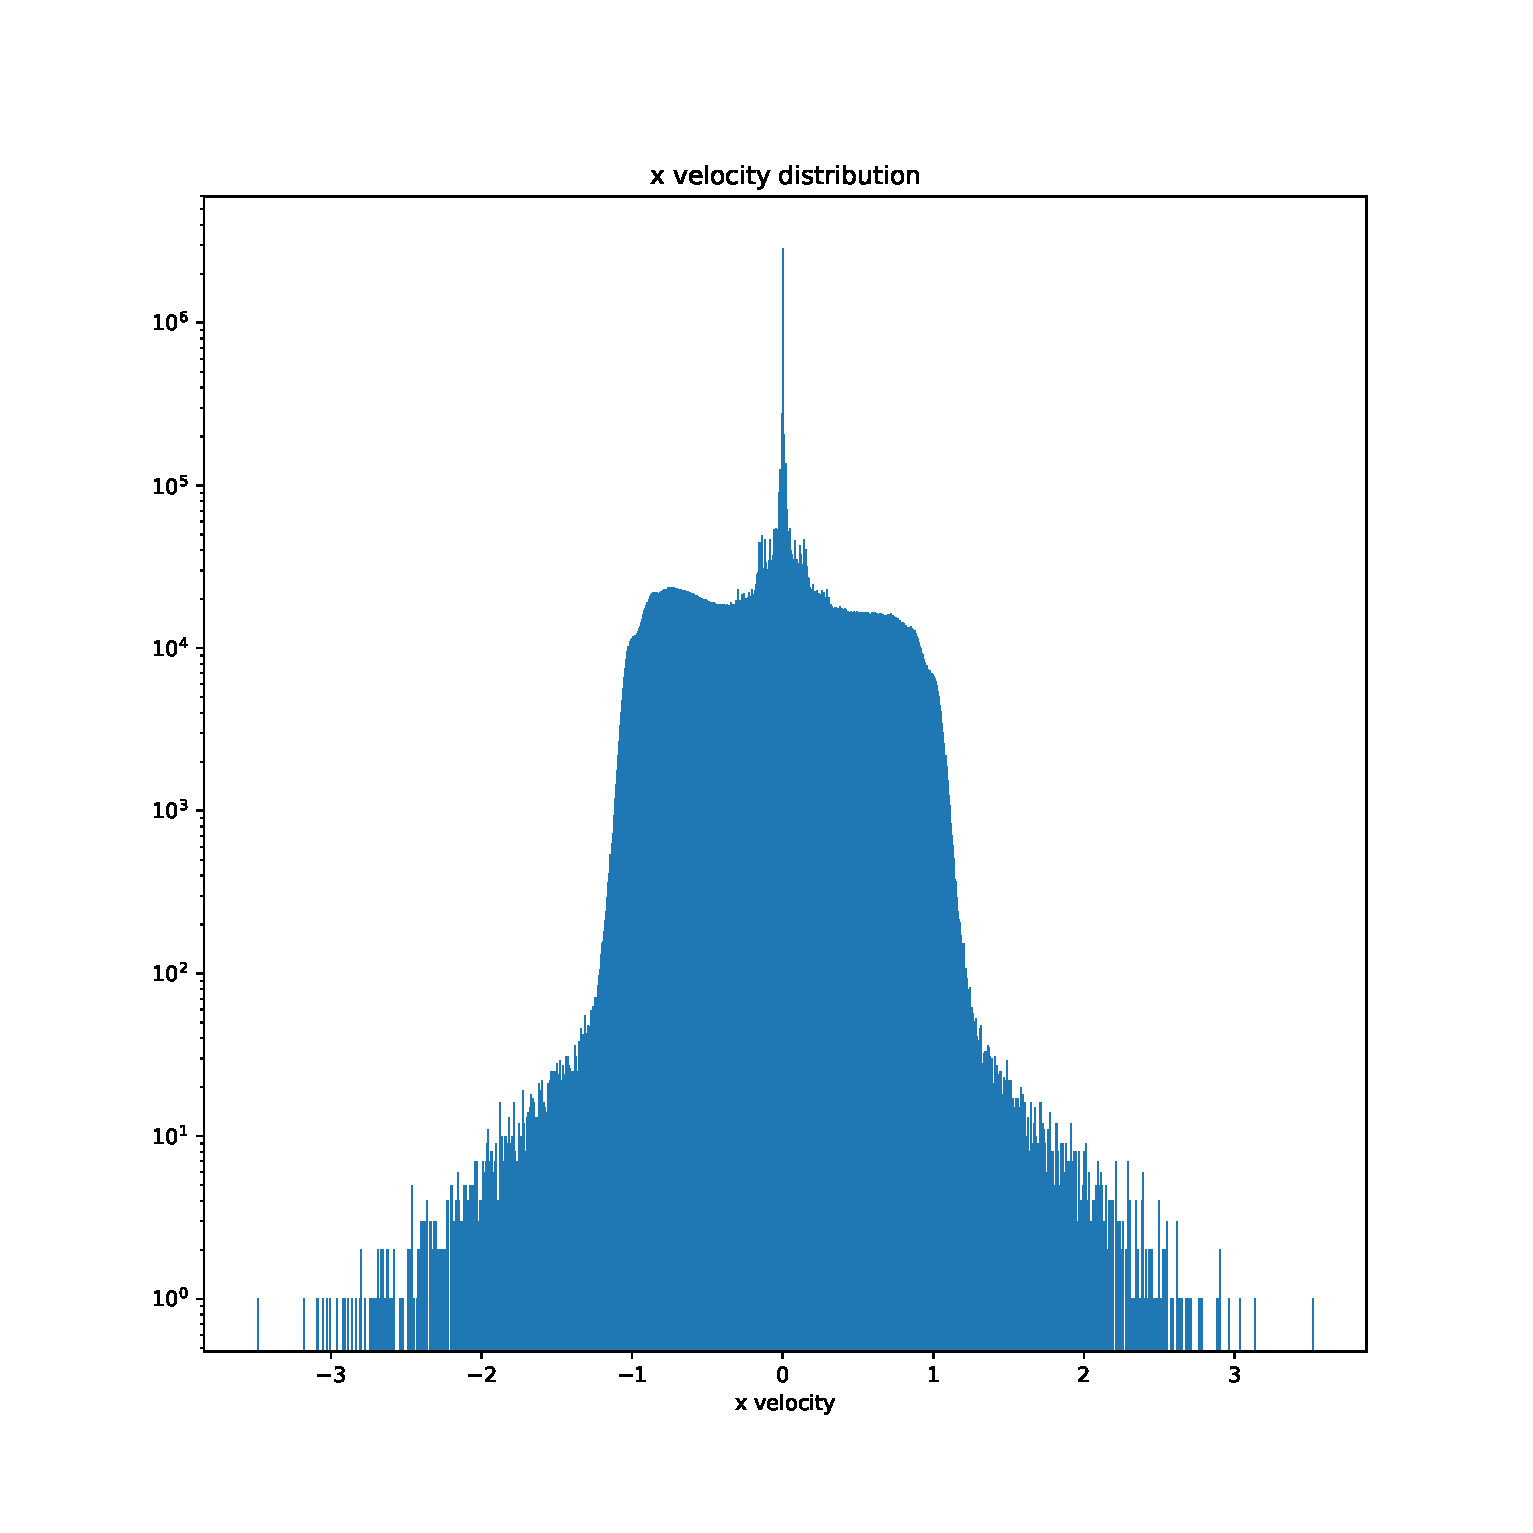
\includegraphics[ width=0.5\textwidth]{/fig/hist_vx/save_trainf10_pro_simTD2Q9_hist_vx}
\captionsetup{width=.8\linewidth}
\caption{CAPTION ONE}
\label{fig:Vx_SimTD2Q9}
\end{minipage}

\begin{minipage}[c]{0.2\linewidth}
\centering
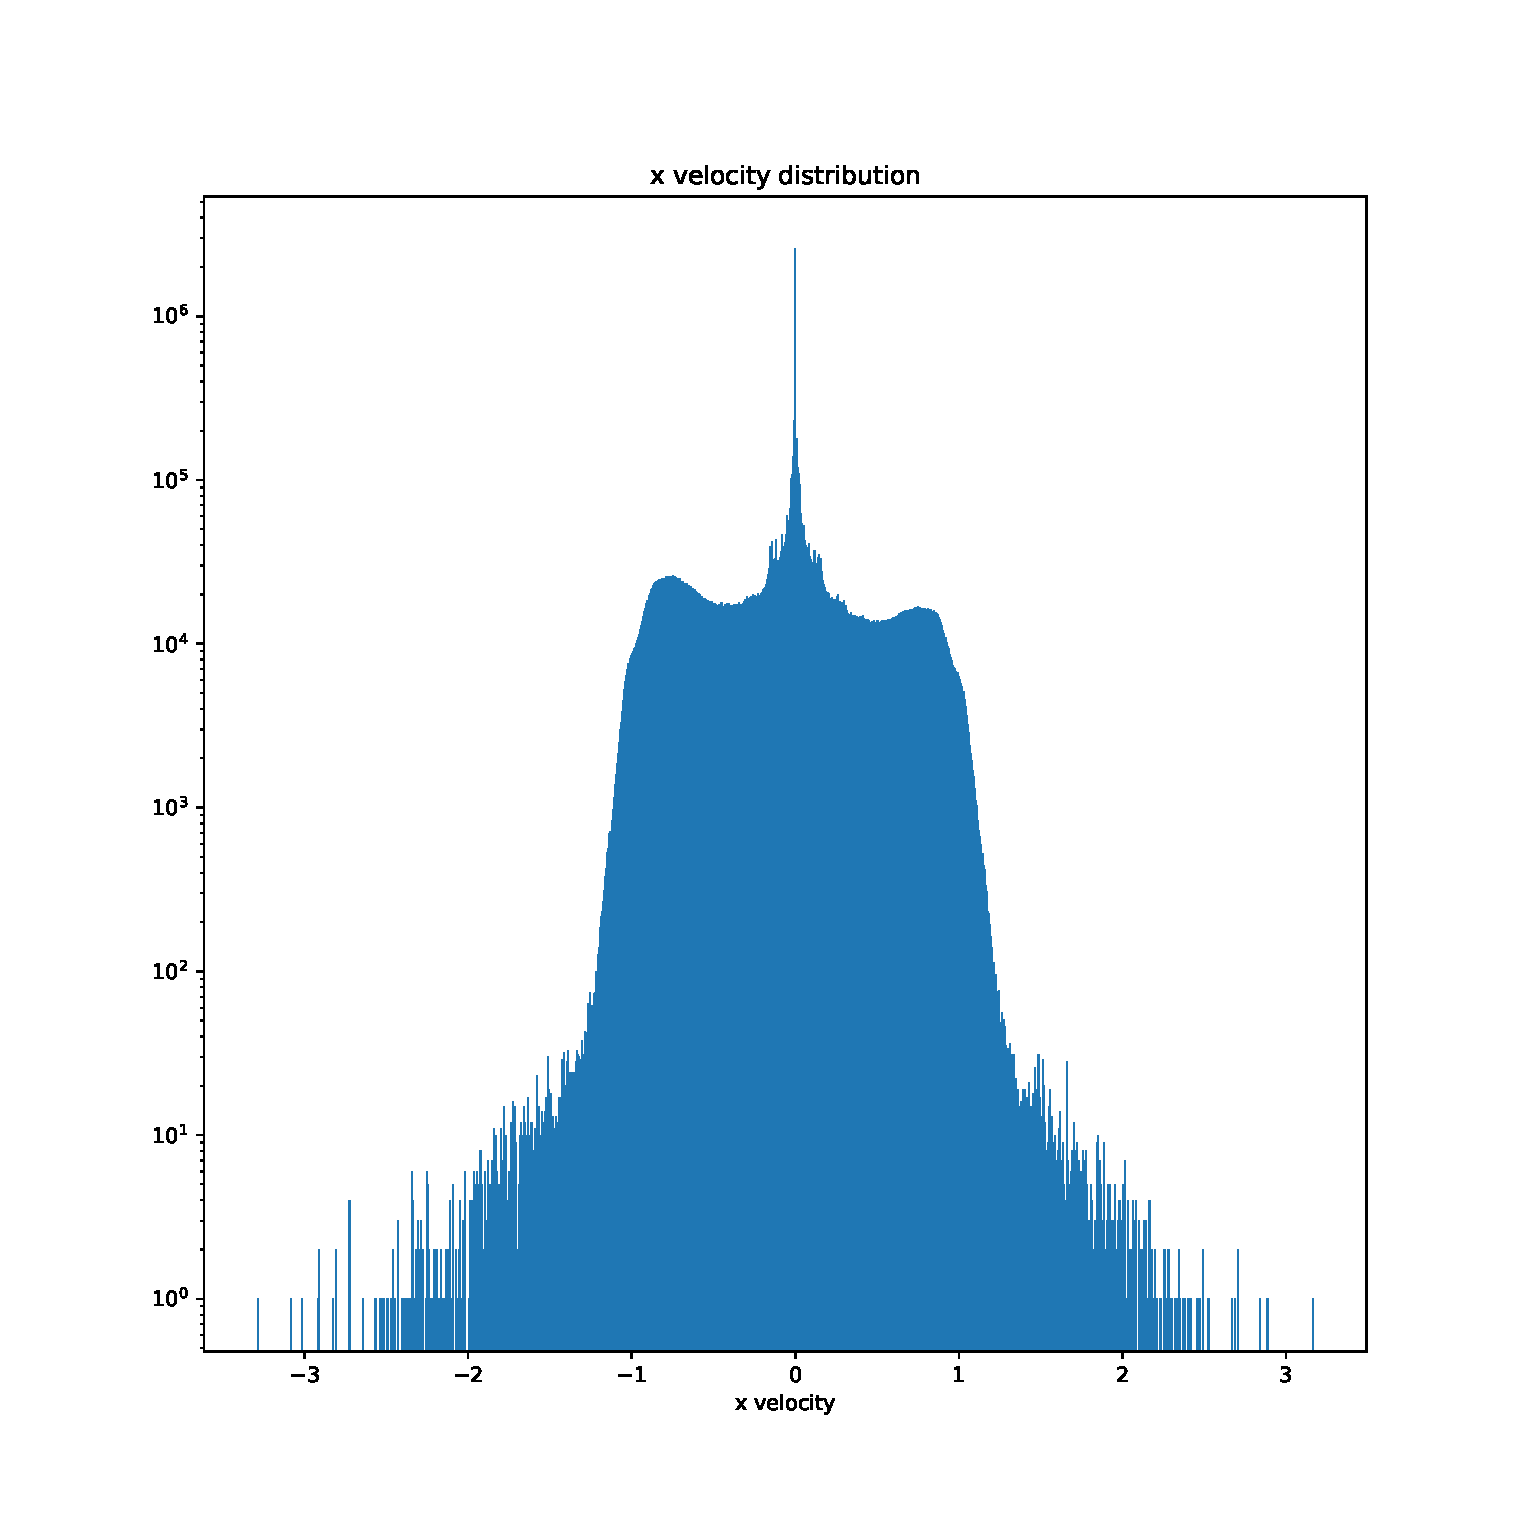
\includegraphics[ width=0.5\textwidth]{/fig/hist_vx/save_trainf10_pro_simTD2Q9Q9_hist_vx}
\captionsetup{width=.8\linewidth}
\caption{CAPTION ONE}
\label{fig:Vx_SimTD2Q9Q9}
\end{minipage}

% ------ ROW ------



% ------ ROW ------



\end{figure}



\FloatBarrier
\end{document}
